% DRAFT: AI-assisted, author must verify every statement, number and reference before submission.
% TODO (authors): this is a plain `article` skeleton. Port to the Springer LNEE / Springer Nature proceedings
% LaTeX template required by the venue before submission (not bundled here); check the 10-page limit after porting.
% TODO (authors): check every entry in refs.bib against the actual publication; entries marked [VERIFY] have
% incomplete author lists.
\documentclass[10pt]{article}
\usepackage[margin=2.5cm]{geometry}
\usepackage{graphicx,booktabs,amsmath,amssymb,hyperref,xcolor}
\graphicspath{{../results/figures/}}
% AUTO-GENERATED by paper/make_numbers.py from results/ -- do not edit by hand
\makeatletter
\newcommand{\R}[2]{\@ifundefined{r@#1@#2}{\textbf{??}}{\csname r@#1@#2\endcsname}}
\newcommand{\V}[2]{\@ifundefined{v@#1@#2}{\textbf{??}}{\csname v@#1@#2\endcsname}}
\newcommand{\D}[1]{\@ifundefined{d@#1}{\textbf{??}}{\csname d@#1\endcsname}}
\makeatother
\expandafter\def\csname r@observed@rate_frac\endcsname{0.024}
\expandafter\def\csname r@observed@phen_frac\endcsname{0.040}
\expandafter\def\csname r@observed@range_frac\endcsname{0.000}
\expandafter\def\csname r@observed@members\endcsname{0}
\expandafter\def\csname r@persistence@mae\endcsname{0.125}
\expandafter\def\csname r@persistence@rmse\endcsname{0.192}
\expandafter\def\csname r@persistence@crps\endcsname{0.125}
\expandafter\def\csname r@persistence@ssim\endcsname{0.613}
\expandafter\def\csname r@persistence@grad_ratio\endcsname{1.07}
\expandafter\def\csname r@persistence@hf_ratio\endcsname{1.14}
\expandafter\def\csname r@persistence@rate_frac\endcsname{0.000}
\expandafter\def\csname r@persistence@phen_frac\endcsname{0.053}
\expandafter\def\csname r@persistence@range_frac\endcsname{0.000}
\expandafter\def\csname r@persistence@members\endcsname{1}
\expandafter\def\csname r@climatology@mae\endcsname{0.120}
\expandafter\def\csname r@climatology@rmse\endcsname{0.176}
\expandafter\def\csname r@climatology@crps\endcsname{0.120}
\expandafter\def\csname r@climatology@ssim\endcsname{0.553}
\expandafter\def\csname r@climatology@grad_ratio\endcsname{0.93}
\expandafter\def\csname r@climatology@hf_ratio\endcsname{1.20}
\expandafter\def\csname r@climatology@rate_frac\endcsname{0.024}
\expandafter\def\csname r@climatology@phen_frac\endcsname{0.023}
\expandafter\def\csname r@climatology@range_frac\endcsname{0.000}
\expandafter\def\csname r@climatology@members\endcsname{1}
\expandafter\def\csname r@clim_anomaly@mae\endcsname{0.150}
\expandafter\def\csname r@clim_anomaly@rmse\endcsname{0.216}
\expandafter\def\csname r@clim_anomaly@crps\endcsname{0.150}
\expandafter\def\csname r@clim_anomaly@ssim\endcsname{0.489}
\expandafter\def\csname r@clim_anomaly@grad_ratio\endcsname{1.44}
\expandafter\def\csname r@clim_anomaly@hf_ratio\endcsname{1.21}
\expandafter\def\csname r@clim_anomaly@rate_frac\endcsname{0.019}
\expandafter\def\csname r@clim_anomaly@phen_frac\endcsname{0.087}
\expandafter\def\csname r@clim_anomaly@range_frac\endcsname{0.032}
\expandafter\def\csname r@clim_anomaly@members\endcsname{1}
\expandafter\def\csname r@det@mae\endcsname{0.104}
\expandafter\def\csname r@det@rmse\endcsname{0.143}
\expandafter\def\csname r@det@crps\endcsname{0.104}
\expandafter\def\csname r@det@ssim\endcsname{0.607}
\expandafter\def\csname r@det@grad_ratio\endcsname{0.64}
\expandafter\def\csname r@det@hf_ratio\endcsname{0.61}
\expandafter\def\csname r@det@rate_frac\endcsname{0.000}
\expandafter\def\csname r@det@phen_frac\endcsname{0.015}
\expandafter\def\csname r@det@mono_frac\endcsname{0.161}
\expandafter\def\csname r@det@range_frac\endcsname{0.000}
\expandafter\def\csname r@det@members\endcsname{1}
\expandafter\def\csname r@diff_plain@mae\endcsname{0.113}
\expandafter\def\csname r@diff_plain@rmse\endcsname{0.158}
\expandafter\def\csname r@diff_plain@crps\endcsname{0.078}
\expandafter\def\csname r@diff_plain@ssim\endcsname{0.327}
\expandafter\def\csname r@diff_plain@grad_ratio\endcsname{1.78}
\expandafter\def\csname r@diff_plain@hf_ratio\endcsname{1.54}
\expandafter\def\csname r@diff_plain@rate_frac\endcsname{0.032}
\expandafter\def\csname r@diff_plain@phen_frac\endcsname{0.060}
\expandafter\def\csname r@diff_plain@mono_frac\endcsname{0.058}
\expandafter\def\csname r@diff_plain@range_frac\endcsname{0.028}
\expandafter\def\csname r@diff_plain@cov50\endcsname{0.431}
\expandafter\def\csname r@diff_plain@cov80\endcsname{0.670}
\expandafter\def\csname r@diff_plain@cov90\endcsname{0.737}
\expandafter\def\csname r@diff_plain@spread_skill\endcsname{0.89}
\expandafter\def\csname r@diff_plain@members\endcsname{8}
\expandafter\def\csname r@diff_phys_G_P@mae\endcsname{0.115}
\expandafter\def\csname r@diff_phys_G_P@rmse\endcsname{0.161}
\expandafter\def\csname r@diff_phys_G_P@crps\endcsname{0.082}
\expandafter\def\csname r@diff_phys_G_P@ssim\endcsname{0.333}
\expandafter\def\csname r@diff_phys_G_P@grad_ratio\endcsname{1.65}
\expandafter\def\csname r@diff_phys_G_P@hf_ratio\endcsname{1.59}
\expandafter\def\csname r@diff_phys_G_P@rate_frac\endcsname{0.000}
\expandafter\def\csname r@diff_phys_G_P@phen_frac\endcsname{0.000}
\expandafter\def\csname r@diff_phys_G_P@mono_frac\endcsname{0.018}
\expandafter\def\csname r@diff_phys_G_P@range_frac\endcsname{0.000}
\expandafter\def\csname r@diff_phys_G_P@cov50\endcsname{0.371}
\expandafter\def\csname r@diff_phys_G_P@cov80\endcsname{0.597}
\expandafter\def\csname r@diff_phys_G_P@cov90\endcsname{0.668}
\expandafter\def\csname r@diff_phys_G_P@spread_skill\endcsname{0.74}
\expandafter\def\csname r@diff_phys_G_P@members\endcsname{8}
\expandafter\def\csname r@diff_phys@mae\endcsname{0.115}
\expandafter\def\csname r@diff_phys@rmse\endcsname{0.162}
\expandafter\def\csname r@diff_phys@crps\endcsname{0.081}
\expandafter\def\csname r@diff_phys@ssim\endcsname{0.320}
\expandafter\def\csname r@diff_phys@grad_ratio\endcsname{1.79}
\expandafter\def\csname r@diff_phys@hf_ratio\endcsname{1.74}
\expandafter\def\csname r@diff_phys@rate_frac\endcsname{0.022}
\expandafter\def\csname r@diff_phys@phen_frac\endcsname{0.040}
\expandafter\def\csname r@diff_phys@mono_frac\endcsname{0.021}
\expandafter\def\csname r@diff_phys@range_frac\endcsname{0.019}
\expandafter\def\csname r@diff_phys@cov50\endcsname{0.394}
\expandafter\def\csname r@diff_phys@cov80\endcsname{0.627}
\expandafter\def\csname r@diff_phys@cov90\endcsname{0.698}
\expandafter\def\csname r@diff_phys@spread_skill\endcsname{0.81}
\expandafter\def\csname r@diff_phys@members\endcsname{8}
\expandafter\def\csname r@diff_phys_G@mae\endcsname{0.115}
\expandafter\def\csname r@diff_phys_G@rmse\endcsname{0.161}
\expandafter\def\csname r@diff_phys_G@crps\endcsname{0.082}
\expandafter\def\csname r@diff_phys_G@ssim\endcsname{0.333}
\expandafter\def\csname r@diff_phys_G@grad_ratio\endcsname{1.65}
\expandafter\def\csname r@diff_phys_G@hf_ratio\endcsname{1.59}
\expandafter\def\csname r@diff_phys_G@rate_frac\endcsname{0.002}
\expandafter\def\csname r@diff_phys_G@phen_frac\endcsname{0.000}
\expandafter\def\csname r@diff_phys_G@mono_frac\endcsname{0.018}
\expandafter\def\csname r@diff_phys_G@range_frac\endcsname{0.000}
\expandafter\def\csname r@diff_phys_G@cov50\endcsname{0.371}
\expandafter\def\csname r@diff_phys_G@cov80\endcsname{0.596}
\expandafter\def\csname r@diff_phys_G@cov90\endcsname{0.668}
\expandafter\def\csname r@diff_phys_G@spread_skill\endcsname{0.74}
\expandafter\def\csname r@diff_phys_G@members\endcsname{8}
\expandafter\def\csname r@diff_phys_P@mae\endcsname{0.114}
\expandafter\def\csname r@diff_phys_P@rmse\endcsname{0.161}
\expandafter\def\csname r@diff_phys_P@crps\endcsname{0.081}
\expandafter\def\csname r@diff_phys_P@ssim\endcsname{0.326}
\expandafter\def\csname r@diff_phys_P@grad_ratio\endcsname{1.73}
\expandafter\def\csname r@diff_phys_P@hf_ratio\endcsname{1.65}
\expandafter\def\csname r@diff_phys_P@rate_frac\endcsname{0.000}
\expandafter\def\csname r@diff_phys_P@phen_frac\endcsname{0.031}
\expandafter\def\csname r@diff_phys_P@mono_frac\endcsname{0.020}
\expandafter\def\csname r@diff_phys_P@range_frac\endcsname{0.000}
\expandafter\def\csname r@diff_phys_P@cov50\endcsname{0.389}
\expandafter\def\csname r@diff_phys_P@cov80\endcsname{0.621}
\expandafter\def\csname r@diff_phys_P@cov90\endcsname{0.693}
\expandafter\def\csname r@diff_phys_P@spread_skill\endcsname{0.78}
\expandafter\def\csname r@diff_phys_P@members\endcsname{8}
\expandafter\def\csname r@diff_plain_G_P@mae\endcsname{0.112}
\expandafter\def\csname r@diff_plain_G_P@rmse\endcsname{0.157}
\expandafter\def\csname r@diff_plain_G_P@crps\endcsname{0.079}
\expandafter\def\csname r@diff_plain_G_P@ssim\endcsname{0.347}
\expandafter\def\csname r@diff_plain_G_P@grad_ratio\endcsname{1.60}
\expandafter\def\csname r@diff_plain_G_P@hf_ratio\endcsname{1.41}
\expandafter\def\csname r@diff_plain_G_P@rate_frac\endcsname{0.000}
\expandafter\def\csname r@diff_plain_G_P@phen_frac\endcsname{0.000}
\expandafter\def\csname r@diff_plain_G_P@mono_frac\endcsname{0.049}
\expandafter\def\csname r@diff_plain_G_P@range_frac\endcsname{0.000}
\expandafter\def\csname r@diff_plain_G_P@cov50\endcsname{0.397}
\expandafter\def\csname r@diff_plain_G_P@cov80\endcsname{0.627}
\expandafter\def\csname r@diff_plain_G_P@cov90\endcsname{0.696}
\expandafter\def\csname r@diff_plain_G_P@spread_skill\endcsname{0.79}
\expandafter\def\csname r@diff_plain_G_P@members\endcsname{8}
\expandafter\def\csname r@clim_anomaly@maelo\endcsname{0.125}
\expandafter\def\csname r@clim_anomaly@maehi\endcsname{0.171}
\expandafter\def\csname r@clim_anomaly@rmselo\endcsname{0.179}
\expandafter\def\csname r@clim_anomaly@rmsehi\endcsname{0.244}
\expandafter\def\csname r@clim_anomaly@crpslo\endcsname{0.125}
\expandafter\def\csname r@clim_anomaly@crpshi\endcsname{0.171}
\expandafter\def\csname r@climatology@maelo\endcsname{0.099}
\expandafter\def\csname r@climatology@maehi\endcsname{0.139}
\expandafter\def\csname r@climatology@rmselo\endcsname{0.147}
\expandafter\def\csname r@climatology@rmsehi\endcsname{0.198}
\expandafter\def\csname r@climatology@crpslo\endcsname{0.099}
\expandafter\def\csname r@climatology@crpshi\endcsname{0.139}
\expandafter\def\csname r@det@maelo\endcsname{0.094}
\expandafter\def\csname r@det@maehi\endcsname{0.111}
\expandafter\def\csname r@det@rmselo\endcsname{0.127}
\expandafter\def\csname r@det@rmsehi\endcsname{0.153}
\expandafter\def\csname r@det@crpslo\endcsname{0.094}
\expandafter\def\csname r@det@crpshi\endcsname{0.111}
\expandafter\def\csname r@diff_phys_G_P@maelo\endcsname{0.099}
\expandafter\def\csname r@diff_phys_G_P@maehi\endcsname{0.130}
\expandafter\def\csname r@diff_phys_G_P@rmselo\endcsname{0.138}
\expandafter\def\csname r@diff_phys_G_P@rmsehi\endcsname{0.182}
\expandafter\def\csname r@diff_phys_G_P@crpslo\endcsname{0.069}
\expandafter\def\csname r@diff_phys_G_P@crpshi\endcsname{0.095}
\expandafter\def\csname r@diff_phys_G@maelo\endcsname{0.100}
\expandafter\def\csname r@diff_phys_G@maehi\endcsname{0.130}
\expandafter\def\csname r@diff_phys_G@rmselo\endcsname{0.138}
\expandafter\def\csname r@diff_phys_G@rmsehi\endcsname{0.182}
\expandafter\def\csname r@diff_phys_G@crpslo\endcsname{0.069}
\expandafter\def\csname r@diff_phys_G@crpshi\endcsname{0.095}
\expandafter\def\csname r@diff_phys_P@maelo\endcsname{0.099}
\expandafter\def\csname r@diff_phys_P@maehi\endcsname{0.130}
\expandafter\def\csname r@diff_phys_P@rmselo\endcsname{0.137}
\expandafter\def\csname r@diff_phys_P@rmsehi\endcsname{0.182}
\expandafter\def\csname r@diff_phys_P@crpslo\endcsname{0.068}
\expandafter\def\csname r@diff_phys_P@crpshi\endcsname{0.094}
\expandafter\def\csname r@diff_phys@maelo\endcsname{0.099}
\expandafter\def\csname r@diff_phys@maehi\endcsname{0.130}
\expandafter\def\csname r@diff_phys@rmselo\endcsname{0.138}
\expandafter\def\csname r@diff_phys@rmsehi\endcsname{0.183}
\expandafter\def\csname r@diff_phys@crpslo\endcsname{0.068}
\expandafter\def\csname r@diff_phys@crpshi\endcsname{0.094}
\expandafter\def\csname r@diff_plain_G_P@maelo\endcsname{0.098}
\expandafter\def\csname r@diff_plain_G_P@maehi\endcsname{0.126}
\expandafter\def\csname r@diff_plain_G_P@rmselo\endcsname{0.135}
\expandafter\def\csname r@diff_plain_G_P@rmsehi\endcsname{0.176}
\expandafter\def\csname r@diff_plain_G_P@crpslo\endcsname{0.068}
\expandafter\def\csname r@diff_plain_G_P@crpshi\endcsname{0.091}
\expandafter\def\csname r@diff_plain@maelo\endcsname{0.098}
\expandafter\def\csname r@diff_plain@maehi\endcsname{0.127}
\expandafter\def\csname r@diff_plain@rmselo\endcsname{0.136}
\expandafter\def\csname r@diff_plain@rmsehi\endcsname{0.178}
\expandafter\def\csname r@diff_plain@crpslo\endcsname{0.067}
\expandafter\def\csname r@diff_plain@crpshi\endcsname{0.090}
\expandafter\def\csname r@persistence@maelo\endcsname{0.105}
\expandafter\def\csname r@persistence@maehi\endcsname{0.147}
\expandafter\def\csname r@persistence@rmselo\endcsname{0.161}
\expandafter\def\csname r@persistence@rmsehi\endcsname{0.224}
\expandafter\def\csname r@persistence@crpslo\endcsname{0.105}
\expandafter\def\csname r@persistence@crpshi\endcsname{0.147}
\expandafter\def\csname r@diffclim_anomaly@mae\endcsname{-0.0358}
\expandafter\def\csname r@diffclim_anomaly@maelo\endcsname{-0.0477}
\expandafter\def\csname r@diffclim_anomaly@maehi\endcsname{-0.0219}
\expandafter\def\csname r@diffclim_anomaly@crps\endcsname{-0.0684}
\expandafter\def\csname r@diffclim_anomaly@crpslo\endcsname{-0.0806}
\expandafter\def\csname r@diffclim_anomaly@crpshi\endcsname{-0.0532}
\expandafter\def\csname r@diffclimatology@mae\endcsname{-0.0053}
\expandafter\def\csname r@diffclimatology@maelo\endcsname{-0.0225}
\expandafter\def\csname r@diffclimatology@maehi\endcsname{0.0138}
\expandafter\def\csname r@diffclimatology@crps\endcsname{-0.0379}
\expandafter\def\csname r@diffclimatology@crpslo\endcsname{-0.0546}
\expandafter\def\csname r@diffclimatology@crpshi\endcsname{-0.0193}
\expandafter\def\csname r@diffdet@mae\endcsname{0.0110}
\expandafter\def\csname r@diffdet@maelo\endcsname{0.0014}
\expandafter\def\csname r@diffdet@maehi\endcsname{0.0209}
\expandafter\def\csname r@diffdet@crps\endcsname{-0.0216}
\expandafter\def\csname r@diffdet@crpslo\endcsname{-0.0298}
\expandafter\def\csname r@diffdet@crpshi\endcsname{-0.0131}
\expandafter\def\csname r@diffdiff_phys_G@mae\endcsname{-0.0001}
\expandafter\def\csname r@diffdiff_phys_G@maelo\endcsname{-0.0001}
\expandafter\def\csname r@diffdiff_phys_G@maehi\endcsname{-0.0000}
\expandafter\def\csname r@diffdiff_phys_G@crps\endcsname{-0.0000}
\expandafter\def\csname r@diffdiff_phys_G@crpslo\endcsname{-0.0001}
\expandafter\def\csname r@diffdiff_phys_G@crpshi\endcsname{-0.0000}
\expandafter\def\csname r@diffdiff_phys_P@mae\endcsname{0.0004}
\expandafter\def\csname r@diffdiff_phys_P@maelo\endcsname{-0.0003}
\expandafter\def\csname r@diffdiff_phys_P@maehi\endcsname{0.0012}
\expandafter\def\csname r@diffdiff_phys_P@crps\endcsname{0.0011}
\expandafter\def\csname r@diffdiff_phys_P@crpslo\endcsname{0.0005}
\expandafter\def\csname r@diffdiff_phys_P@crpshi\endcsname{0.0019}
\expandafter\def\csname r@diffdiff_phys@mae\endcsname{-0.0005}
\expandafter\def\csname r@diffdiff_phys@maelo\endcsname{-0.0011}
\expandafter\def\csname r@diffdiff_phys@maehi\endcsname{0.0004}
\expandafter\def\csname r@diffdiff_phys@crps\endcsname{0.0008}
\expandafter\def\csname r@diffdiff_phys@crpslo\endcsname{0.0002}
\expandafter\def\csname r@diffdiff_phys@crpshi\endcsname{0.0017}
\expandafter\def\csname r@diffdiff_plain_G_P@mae\endcsname{0.0028}
\expandafter\def\csname r@diffdiff_plain_G_P@maelo\endcsname{0.0006}
\expandafter\def\csname r@diffdiff_plain_G_P@maehi\endcsname{0.0049}
\expandafter\def\csname r@diffdiff_plain_G_P@crps\endcsname{0.0029}
\expandafter\def\csname r@diffdiff_plain_G_P@crpslo\endcsname{0.0011}
\expandafter\def\csname r@diffdiff_plain_G_P@crpshi\endcsname{0.0047}
\expandafter\def\csname r@diffdiff_plain@mae\endcsname{0.0020}
\expandafter\def\csname r@diffdiff_plain@maelo\endcsname{-0.0004}
\expandafter\def\csname r@diffdiff_plain@maehi\endcsname{0.0041}
\expandafter\def\csname r@diffdiff_plain@crps\endcsname{0.0037}
\expandafter\def\csname r@diffdiff_plain@crpslo\endcsname{0.0016}
\expandafter\def\csname r@diffdiff_plain@crpshi\endcsname{0.0057}
\expandafter\def\csname r@diffpersistence@mae\endcsname{-0.0110}
\expandafter\def\csname r@diffpersistence@maelo\endcsname{-0.0204}
\expandafter\def\csname r@diffpersistence@maehi\endcsname{-0.0003}
\expandafter\def\csname r@diffpersistence@crps\endcsname{-0.0436}
\expandafter\def\csname r@diffpersistence@crpslo\endcsname{-0.0540}
\expandafter\def\csname r@diffpersistence@crpshi\endcsname{-0.0320}
\expandafter\def\csname v@clim_anomaly@mae_nondrought\endcsname{0.151}
\expandafter\def\csname v@climatology@mae_nondrought\endcsname{0.120}
\expandafter\def\csname v@det@mae_nondrought\endcsname{0.107}
\expandafter\def\csname v@diff_phys_G_P@mae_nondrought\endcsname{0.117}
\expandafter\def\csname v@diff_phys_G@mae_nondrought\endcsname{0.117}
\expandafter\def\csname v@diff_phys_P@mae_nondrought\endcsname{0.117}
\expandafter\def\csname v@diff_phys@mae_nondrought\endcsname{0.118}
\expandafter\def\csname v@diff_plain_G_P@mae_nondrought\endcsname{0.116}
\expandafter\def\csname v@diff_plain@mae_nondrought\endcsname{0.116}
\expandafter\def\csname v@persistence@mae_nondrought\endcsname{0.130}
\expandafter\def\csname v@det@mae_normalD\endcsname{0.095}
\expandafter\def\csname v@det@mae_persistenceD\endcsname{0.083}
\expandafter\def\csname v@det@mae_climatologyD\endcsname{0.073}
\expandafter\def\csname v@det@mae_factualD\endcsname{0.101}
\expandafter\def\csname v@det@mae_normalA\endcsname{0.120}
\expandafter\def\csname v@det@mae_persistenceA\endcsname{0.100}
\expandafter\def\csname v@det@mae_climatologyA\endcsname{0.084}
\expandafter\def\csname v@det@mae_factualA\endcsname{0.122}
\expandafter\def\csname v@diff_phys@mae_normalD\endcsname{0.121}
\expandafter\def\csname v@diff_phys@mae_persistenceD\endcsname{0.083}
\expandafter\def\csname v@diff_phys@mae_climatologyD\endcsname{0.073}
\expandafter\def\csname v@diff_phys@mae_factualD\endcsname{0.111}
\expandafter\def\csname v@diff_phys@mae_normalA\endcsname{0.132}
\expandafter\def\csname v@diff_phys@mae_persistenceA\endcsname{0.100}
\expandafter\def\csname v@diff_phys@mae_climatologyA\endcsname{0.084}
\expandafter\def\csname v@diff_phys@mae_factualA\endcsname{0.130}
\expandafter\def\csname v@diff_phys_G_P@mae_normalD\endcsname{0.123}
\expandafter\def\csname v@diff_phys_G_P@mae_persistenceD\endcsname{0.083}
\expandafter\def\csname v@diff_phys_G_P@mae_climatologyD\endcsname{0.073}
\expandafter\def\csname v@diff_phys_G_P@mae_factualD\endcsname{0.110}
\expandafter\def\csname v@diff_phys_G_P@mae_normalA\endcsname{0.134}
\expandafter\def\csname v@diff_phys_G_P@mae_persistenceA\endcsname{0.100}
\expandafter\def\csname v@diff_phys_G_P@mae_climatologyA\endcsname{0.084}
\expandafter\def\csname v@diff_phys_G_P@mae_factualA\endcsname{0.132}
\expandafter\def\csname v@diff_phys_G_P_C@mae_normalD\endcsname{0.123}
\expandafter\def\csname v@diff_phys_G_P_C@mae_persistenceD\endcsname{0.083}
\expandafter\def\csname v@diff_phys_G_P_C@mae_climatologyD\endcsname{0.073}
\expandafter\def\csname v@diff_phys_G_P_C@mae_factualD\endcsname{0.110}
\expandafter\def\csname v@diff_phys_G_P_C@mae_normalA\endcsname{0.134}
\expandafter\def\csname v@diff_phys_G_P_C@mae_persistenceA\endcsname{0.100}
\expandafter\def\csname v@diff_phys_G_P_C@mae_climatologyA\endcsname{0.084}
\expandafter\def\csname v@diff_phys_G_P_C@mae_factualA\endcsname{0.132}
\expandafter\def\csname v@diff_plain@mae_normalD\endcsname{0.106}
\expandafter\def\csname v@diff_plain@mae_persistenceD\endcsname{0.083}
\expandafter\def\csname v@diff_plain@mae_climatologyD\endcsname{0.073}
\expandafter\def\csname v@diff_plain@mae_factualD\endcsname{0.106}
\expandafter\def\csname v@diff_plain@mae_normalA\endcsname{0.125}
\expandafter\def\csname v@diff_plain@mae_persistenceA\endcsname{0.100}
\expandafter\def\csname v@diff_plain@mae_climatologyA\endcsname{0.084}
\expandafter\def\csname v@diff_plain@mae_factualA\endcsname{0.126}
\expandafter\def\csname v@det@n_matched\endcsname{5}
\expandafter\def\csname v@det@max_abs_smd\endcsname{0.380}
\expandafter\def\csname v@det@did_mean\endcsname{0.002}
\expandafter\def\csname v@det@model_mean\endcsname{-0.020}
\expandafter\def\csname v@det@bias_model_minus_did\endcsname{-0.022}
\expandafter\def\csname v@det@corr\endcsname{0.009}
\expandafter\def\csname v@det@did_in_model_90pi\endcsname{0.000}
\expandafter\def\csname v@det@anom_n\endcsname{80}
\expandafter\def\csname v@det@anom_corr\endcsname{0.140}
\expandafter\def\csname v@det@anom_corr_lo95\endcsname{-0.195}
\expandafter\def\csname v@det@anom_corr_hi95\endcsname{0.391}
\expandafter\def\csname v@det@anom_slope\endcsname{0.443}
\expandafter\def\csname v@det@anom_mean_obs_drought\endcsname{-0.023}
\expandafter\def\csname v@det@anom_mean_model_drought\endcsname{-0.022}
\expandafter\def\csname v@diff_phys@n_matched\endcsname{5}
\expandafter\def\csname v@diff_phys@max_abs_smd\endcsname{0.380}
\expandafter\def\csname v@diff_phys@did_mean\endcsname{0.002}
\expandafter\def\csname v@diff_phys@model_mean\endcsname{-0.059}
\expandafter\def\csname v@diff_phys@bias_model_minus_did\endcsname{-0.061}
\expandafter\def\csname v@diff_phys@corr\endcsname{-0.573}
\expandafter\def\csname v@diff_phys@did_in_model_90pi\endcsname{0.000}
\expandafter\def\csname v@diff_phys@anom_n\endcsname{80}
\expandafter\def\csname v@diff_phys@anom_corr\endcsname{0.153}
\expandafter\def\csname v@diff_phys@anom_corr_lo95\endcsname{-0.053}
\expandafter\def\csname v@diff_phys@anom_corr_hi95\endcsname{0.420}
\expandafter\def\csname v@diff_phys@anom_slope\endcsname{0.338}
\expandafter\def\csname v@diff_phys@anom_mean_obs_drought\endcsname{-0.023}
\expandafter\def\csname v@diff_phys@anom_mean_model_drought\endcsname{-0.056}
\expandafter\def\csname v@diff_phys_G_P@n_matched\endcsname{5}
\expandafter\def\csname v@diff_phys_G_P@max_abs_smd\endcsname{0.380}
\expandafter\def\csname v@diff_phys_G_P@did_mean\endcsname{0.002}
\expandafter\def\csname v@diff_phys_G_P@model_mean\endcsname{-0.059}
\expandafter\def\csname v@diff_phys_G_P@bias_model_minus_did\endcsname{-0.062}
\expandafter\def\csname v@diff_phys_G_P@corr\endcsname{-0.559}
\expandafter\def\csname v@diff_phys_G_P@did_in_model_90pi\endcsname{0.000}
\expandafter\def\csname v@diff_phys_G_P@anom_n\endcsname{80}
\expandafter\def\csname v@diff_phys_G_P@anom_corr\endcsname{0.158}
\expandafter\def\csname v@diff_phys_G_P@anom_corr_lo95\endcsname{-0.051}
\expandafter\def\csname v@diff_phys_G_P@anom_corr_hi95\endcsname{0.430}
\expandafter\def\csname v@diff_phys_G_P@anom_slope\endcsname{0.352}
\expandafter\def\csname v@diff_phys_G_P@anom_mean_obs_drought\endcsname{-0.023}
\expandafter\def\csname v@diff_phys_G_P@anom_mean_model_drought\endcsname{-0.061}
\expandafter\def\csname v@diff_phys_G_P_C@n_matched\endcsname{5}
\expandafter\def\csname v@diff_phys_G_P_C@max_abs_smd\endcsname{0.380}
\expandafter\def\csname v@diff_phys_G_P_C@did_mean\endcsname{0.002}
\expandafter\def\csname v@diff_phys_G_P_C@model_mean\endcsname{-0.059}
\expandafter\def\csname v@diff_phys_G_P_C@bias_model_minus_did\endcsname{-0.062}
\expandafter\def\csname v@diff_phys_G_P_C@corr\endcsname{-0.559}
\expandafter\def\csname v@diff_phys_G_P_C@did_in_model_90pi\endcsname{0.000}
\expandafter\def\csname v@diff_phys_G_P_C@anom_n\endcsname{80}
\expandafter\def\csname v@diff_phys_G_P_C@anom_corr\endcsname{0.158}
\expandafter\def\csname v@diff_phys_G_P_C@anom_corr_lo95\endcsname{-0.051}
\expandafter\def\csname v@diff_phys_G_P_C@anom_corr_hi95\endcsname{0.430}
\expandafter\def\csname v@diff_phys_G_P_C@anom_slope\endcsname{0.352}
\expandafter\def\csname v@diff_phys_G_P_C@anom_mean_obs_drought\endcsname{-0.023}
\expandafter\def\csname v@diff_phys_G_P_C@anom_mean_model_drought\endcsname{-0.061}
\expandafter\def\csname v@diff_plain@n_matched\endcsname{5}
\expandafter\def\csname v@diff_plain@max_abs_smd\endcsname{0.380}
\expandafter\def\csname v@diff_plain@did_mean\endcsname{0.002}
\expandafter\def\csname v@diff_plain@model_mean\endcsname{-0.040}
\expandafter\def\csname v@diff_plain@bias_model_minus_did\endcsname{-0.042}
\expandafter\def\csname v@diff_plain@corr\endcsname{-0.419}
\expandafter\def\csname v@diff_plain@did_in_model_90pi\endcsname{0.000}
\expandafter\def\csname v@diff_plain@anom_n\endcsname{80}
\expandafter\def\csname v@diff_plain@anom_corr\endcsname{0.112}
\expandafter\def\csname v@diff_plain@anom_corr_lo95\endcsname{-0.069}
\expandafter\def\csname v@diff_plain@anom_corr_hi95\endcsname{0.364}
\expandafter\def\csname v@diff_plain@anom_slope\endcsname{0.219}
\expandafter\def\csname v@diff_plain@anom_mean_obs_drought\endcsname{-0.023}
\expandafter\def\csname v@diff_plain@anom_mean_model_drought\endcsname{-0.039}
\expandafter\def\csname v@det@scenario_placebo_mean\endcsname{0.000}
\expandafter\def\csname v@det@noise_placebo_mean\endcsname{0.000}
\expandafter\def\csname v@det@scenario_placebo_frac_below_tol\endcsname{1.000}
\expandafter\def\csname v@det@temporal_auc\endcsname{0.692}
\expandafter\def\csname v@det@perm_real_contrast\endcsname{-0.014}
\expandafter\def\csname v@det@perm_null_mean\endcsname{-0.002}
\expandafter\def\csname v@det@perm_p_one_sided\endcsname{0.064}
\expandafter\def\csname v@det@crn_var_ratio\endcsname{0.886}
\expandafter\def\csname v@det@frac_drought_above_normal\endcsname{0.194}
\expandafter\def\csname v@det@mean_dDN_drought_windows\endcsname{-0.022}
\expandafter\def\csname v@diff_phys@scenario_placebo_mean\endcsname{-0.000}
\expandafter\def\csname v@diff_phys@noise_placebo_mean\endcsname{0.001}
\expandafter\def\csname v@diff_phys@scenario_placebo_frac_below_tol\endcsname{1.000}
\expandafter\def\csname v@diff_phys@temporal_auc\endcsname{0.942}
\expandafter\def\csname v@diff_phys@perm_real_contrast\endcsname{-0.055}
\expandafter\def\csname v@diff_phys@perm_null_mean\endcsname{-0.013}
\expandafter\def\csname v@diff_phys@perm_p_one_sided\endcsname{0.001}
\expandafter\def\csname v@diff_phys@crn_var_ratio\endcsname{0.032}
\expandafter\def\csname v@diff_phys@frac_drought_above_normal\endcsname{0.028}
\expandafter\def\csname v@diff_phys@mean_dDN_drought_windows\endcsname{-0.059}
\expandafter\def\csname v@diff_phys_G_P@scenario_placebo_mean\endcsname{-0.000}
\expandafter\def\csname v@diff_phys_G_P@noise_placebo_mean\endcsname{0.001}
\expandafter\def\csname v@diff_phys_G_P@scenario_placebo_frac_below_tol\endcsname{1.000}
\expandafter\def\csname v@diff_phys_G_P@temporal_auc\endcsname{0.962}
\expandafter\def\csname v@diff_phys_G_P@perm_real_contrast\endcsname{-0.061}
\expandafter\def\csname v@diff_phys_G_P@perm_null_mean\endcsname{-0.013}
\expandafter\def\csname v@diff_phys_G_P@perm_p_one_sided\endcsname{0.001}
\expandafter\def\csname v@diff_phys_G_P@crn_var_ratio\endcsname{0.048}
\expandafter\def\csname v@diff_phys_G_P@frac_drought_above_normal\endcsname{0.024}
\expandafter\def\csname v@diff_phys_G_P@mean_dDN_drought_windows\endcsname{-0.064}
\expandafter\def\csname v@diff_phys_G_P_C@scenario_placebo_mean\endcsname{-0.000}
\expandafter\def\csname v@diff_phys_G_P_C@noise_placebo_mean\endcsname{0.001}
\expandafter\def\csname v@diff_phys_G_P_C@scenario_placebo_frac_below_tol\endcsname{1.000}
\expandafter\def\csname v@diff_phys_G_P_C@temporal_auc\endcsname{0.962}
\expandafter\def\csname v@diff_phys_G_P_C@perm_real_contrast\endcsname{-0.061}
\expandafter\def\csname v@diff_phys_G_P_C@perm_null_mean\endcsname{-0.013}
\expandafter\def\csname v@diff_phys_G_P_C@perm_p_one_sided\endcsname{0.001}
\expandafter\def\csname v@diff_phys_G_P_C@crn_var_ratio\endcsname{0.046}
\expandafter\def\csname v@diff_phys_G_P_C@frac_drought_above_normal\endcsname{0.000}
\expandafter\def\csname v@diff_phys_G_P_C@mean_dDN_drought_windows\endcsname{-0.064}
\expandafter\def\csname v@diff_plain@scenario_placebo_mean\endcsname{0.000}
\expandafter\def\csname v@diff_plain@noise_placebo_mean\endcsname{0.001}
\expandafter\def\csname v@diff_plain@scenario_placebo_frac_below_tol\endcsname{0.981}
\expandafter\def\csname v@diff_plain@temporal_auc\endcsname{0.854}
\expandafter\def\csname v@diff_plain@perm_real_contrast\endcsname{-0.039}
\expandafter\def\csname v@diff_plain@perm_null_mean\endcsname{-0.010}
\expandafter\def\csname v@diff_plain@perm_p_one_sided\endcsname{0.016}
\expandafter\def\csname v@diff_plain@crn_var_ratio\endcsname{0.028}
\expandafter\def\csname v@diff_plain@frac_drought_above_normal\endcsname{0.091}
\expandafter\def\csname v@diff_plain@mean_dDN_drought_windows\endcsname{-0.041}
\expandafter\def\csname v@persistence@crps\endcsname{0.125}
\expandafter\def\csname v@climatology@crps\endcsname{0.120}
\expandafter\def\csname v@clim_anomaly@crps\endcsname{0.150}
\expandafter\def\csname v@det@crps\endcsname{0.104}
\expandafter\def\csname v@det@did_in_effect_90pi\endcsname{0.000}
\expandafter\def\csname v@diff_plain@crps\endcsname{0.078}
\expandafter\def\csname v@diff_plain@cov50\endcsname{0.431}
\expandafter\def\csname v@diff_plain@cov80\endcsname{0.670}
\expandafter\def\csname v@diff_plain@cov90\endcsname{0.737}
\expandafter\def\csname v@diff_plain@spread_skill\endcsname{0.886}
\expandafter\def\csname v@diff_plain@rank_hist_chi2_flatness\endcsname{0.041}
\expandafter\def\csname v@diff_plain@did_in_effect_90pi\endcsname{0.000}
\expandafter\def\csname v@diff_phys+G+P@crps\endcsname{0.082}
\expandafter\def\csname v@diff_phys+G+P@cov50\endcsname{0.371}
\expandafter\def\csname v@diff_phys+G+P@cov80\endcsname{0.597}
\expandafter\def\csname v@diff_phys+G+P@cov90\endcsname{0.668}
\expandafter\def\csname v@diff_phys+G+P@spread_skill\endcsname{0.739}
\expandafter\def\csname v@diff_phys+G+P@rank_hist_chi2_flatness\endcsname{0.087}
\expandafter\def\csname v@diff_phys+G+P@did_in_effect_90pi\endcsname{0.000}
\expandafter\def\csname v@diff_phys@crps\endcsname{0.081}
\expandafter\def\csname v@diff_phys@cov50\endcsname{0.394}
\expandafter\def\csname v@diff_phys@cov80\endcsname{0.627}
\expandafter\def\csname v@diff_phys@cov90\endcsname{0.698}
\expandafter\def\csname v@diff_phys@spread_skill\endcsname{0.805}
\expandafter\def\csname v@diff_phys@rank_hist_chi2_flatness\endcsname{0.063}
\expandafter\def\csname v@diff_phys@did_in_effect_90pi\endcsname{0.000}
\expandafter\def\csname v@diff_phys+G@crps\endcsname{0.082}
\expandafter\def\csname v@diff_phys+G@cov50\endcsname{0.371}
\expandafter\def\csname v@diff_phys+G@cov80\endcsname{0.596}
\expandafter\def\csname v@diff_phys+G@cov90\endcsname{0.668}
\expandafter\def\csname v@diff_phys+G@spread_skill\endcsname{0.739}
\expandafter\def\csname v@diff_phys+G@rank_hist_chi2_flatness\endcsname{0.088}
\expandafter\def\csname v@diff_phys+P@crps\endcsname{0.081}
\expandafter\def\csname v@diff_phys+P@cov50\endcsname{0.389}
\expandafter\def\csname v@diff_phys+P@cov80\endcsname{0.621}
\expandafter\def\csname v@diff_phys+P@cov90\endcsname{0.693}
\expandafter\def\csname v@diff_phys+P@spread_skill\endcsname{0.780}
\expandafter\def\csname v@diff_phys+P@rank_hist_chi2_flatness\endcsname{0.061}
\expandafter\def\csname v@diff_plain+G+P@crps\endcsname{0.079}
\expandafter\def\csname v@diff_plain+G+P@cov50\endcsname{0.397}
\expandafter\def\csname v@diff_plain+G+P@cov80\endcsname{0.627}
\expandafter\def\csname v@diff_plain+G+P@cov90\endcsname{0.696}
\expandafter\def\csname v@diff_plain+G+P@spread_skill\endcsname{0.788}
\expandafter\def\csname v@diff_plain+G+P@rank_hist_chi2_flatness\endcsname{0.062}
\expandafter\def\csname v@observed@rate_frac\endcsname{0.024}
\expandafter\def\csname v@observed@rate_mag\endcsname{0.027}
\expandafter\def\csname v@observed@phen_frac\endcsname{0.040}
\expandafter\def\csname v@observed@phen_mag\endcsname{0.123}
\expandafter\def\csname v@observed@range_frac\endcsname{0.000}
\expandafter\def\csname v@persistence@rate_frac\endcsname{0.000}
\expandafter\def\csname v@persistence@rate_mag\endcsname{0.000}
\expandafter\def\csname v@persistence@phen_frac\endcsname{0.053}
\expandafter\def\csname v@persistence@phen_mag\endcsname{0.120}
\expandafter\def\csname v@persistence@range_frac\endcsname{0.000}
\expandafter\def\csname v@climatology@rate_frac\endcsname{0.024}
\expandafter\def\csname v@climatology@rate_mag\endcsname{0.021}
\expandafter\def\csname v@climatology@phen_frac\endcsname{0.023}
\expandafter\def\csname v@climatology@phen_mag\endcsname{0.104}
\expandafter\def\csname v@climatology@range_frac\endcsname{0.000}
\expandafter\def\csname v@clim_anomaly@rate_frac\endcsname{0.019}
\expandafter\def\csname v@clim_anomaly@rate_mag\endcsname{0.019}
\expandafter\def\csname v@clim_anomaly@phen_frac\endcsname{0.087}
\expandafter\def\csname v@clim_anomaly@phen_mag\endcsname{0.125}
\expandafter\def\csname v@clim_anomaly@range_frac\endcsname{0.032}
\expandafter\def\csname v@det@rate_frac\endcsname{0.000}
\expandafter\def\csname v@det@rate_mag\endcsname{0.011}
\expandafter\def\csname v@det@phen_frac\endcsname{0.015}
\expandafter\def\csname v@det@phen_mag\endcsname{0.088}
\expandafter\def\csname v@det@range_frac\endcsname{0.000}
\expandafter\def\csname v@det@mono_frac\endcsname{0.161}
\expandafter\def\csname v@det@mono_mag\endcsname{0.023}
\expandafter\def\csname v@diff_plain@rate_frac\endcsname{0.032}
\expandafter\def\csname v@diff_plain@rate_mag\endcsname{0.016}
\expandafter\def\csname v@diff_plain@phen_frac\endcsname{0.060}
\expandafter\def\csname v@diff_plain@phen_mag\endcsname{0.079}
\expandafter\def\csname v@diff_plain@range_frac\endcsname{0.028}
\expandafter\def\csname v@diff_plain@mono_frac\endcsname{0.058}
\expandafter\def\csname v@diff_plain@mono_mag\endcsname{0.028}
\expandafter\def\csname v@diff_phys+G+P@rate_frac\endcsname{0.000}
\expandafter\def\csname v@diff_phys+G+P@rate_mag\endcsname{0.000}
\expandafter\def\csname v@diff_phys+G+P@phen_frac\endcsname{0.000}
\expandafter\def\csname v@diff_phys+G+P@phen_mag\endcsname{0.060}
\expandafter\def\csname v@diff_phys+G+P@range_frac\endcsname{0.000}
\expandafter\def\csname v@diff_phys+G+P@mono_frac\endcsname{0.018}
\expandafter\def\csname v@diff_phys+G+P@mono_mag\endcsname{0.016}
\expandafter\def\csname v@diff_phys@rate_frac\endcsname{0.022}
\expandafter\def\csname v@diff_phys@rate_mag\endcsname{0.016}
\expandafter\def\csname v@diff_phys@phen_frac\endcsname{0.040}
\expandafter\def\csname v@diff_phys@phen_mag\endcsname{0.068}
\expandafter\def\csname v@diff_phys@range_frac\endcsname{0.019}
\expandafter\def\csname v@diff_phys@mono_frac\endcsname{0.021}
\expandafter\def\csname v@diff_phys@mono_mag\endcsname{0.017}
\expandafter\def\csname v@diff_phys+G@rate_frac\endcsname{0.002}
\expandafter\def\csname v@diff_phys+G@rate_mag\endcsname{0.004}
\expandafter\def\csname v@diff_phys+G@phen_frac\endcsname{0.000}
\expandafter\def\csname v@diff_phys+G@phen_mag\endcsname{0.022}
\expandafter\def\csname v@diff_phys+G@range_frac\endcsname{0.000}
\expandafter\def\csname v@diff_phys+G@mono_frac\endcsname{0.018}
\expandafter\def\csname v@diff_phys+G@mono_mag\endcsname{0.016}
\expandafter\def\csname v@diff_phys+P@rate_frac\endcsname{0.000}
\expandafter\def\csname v@diff_phys+P@rate_mag\endcsname{0.000}
\expandafter\def\csname v@diff_phys+P@phen_frac\endcsname{0.031}
\expandafter\def\csname v@diff_phys+P@phen_mag\endcsname{0.058}
\expandafter\def\csname v@diff_phys+P@range_frac\endcsname{0.000}
\expandafter\def\csname v@diff_phys+P@mono_frac\endcsname{0.020}
\expandafter\def\csname v@diff_phys+P@mono_mag\endcsname{0.017}
\expandafter\def\csname v@diff_plain+G+P@rate_frac\endcsname{0.000}
\expandafter\def\csname v@diff_plain+G+P@rate_mag\endcsname{0.000}
\expandafter\def\csname v@diff_plain+G+P@phen_frac\endcsname{0.000}
\expandafter\def\csname v@diff_plain+G+P@phen_mag\endcsname{0.059}
\expandafter\def\csname v@diff_plain+G+P@range_frac\endcsname{0.000}
\expandafter\def\csname v@diff_plain+G+P@mono_frac\endcsname{0.049}
\expandafter\def\csname v@diff_plain+G+P@mono_mag\endcsname{0.028}
\expandafter\def\csname d@nloc\endcsname{69}
\expandafter\def\csname d@nloctrain\endcsname{49}
\expandafter\def\csname d@nwintrain\endcsname{2399}
\expandafter\def\csname d@dfractrain\endcsname{0.142}
\expandafter\def\csname d@nlocval\endcsname{10}
\expandafter\def\csname d@nwinval\endcsname{153}
\expandafter\def\csname d@dfracval\endcsname{0.052}
\expandafter\def\csname d@nloctest\endcsname{10}
\expandafter\def\csname d@nwintest\endcsname{270}
\expandafter\def\csname d@dfractest\endcsname{0.126}
\expandafter\def\csname d@validfrac\endcsname{0.496}
\expandafter\def\csname d@rincforest\endcsname{0.062}
\expandafter\def\csname d@rdecforest\endcsname{0.068}
\expandafter\def\csname d@rincgrass\endcsname{0.057}
\expandafter\def\csname d@rdecgrass\endcsname{0.076}
\expandafter\def\csname d@rinccrop\endcsname{0.060}
\expandafter\def\csname d@rdeccrop\endcsname{0.091}
\expandafter\def\csname d@rincother\endcsname{0.063}
\expandafter\def\csname d@rdecother\endcsname{0.064}
\expandafter\def\csname d@sharpness_closeness_diff_phys_G_P\endcsname{0.962}
\expandafter\def\csname d@sharpness_closeness_det\endcsname{0.943}
\expandafter\def\csname d@sharpness_closeness_diff_plain\endcsname{1.010}
\expandafter\def\csname d@anom_ratio_diff_phys_G_P\endcsname{2.7}
\expandafter\def\csname d@anom_ratio_diff_phys\endcsname{2.5}
\expandafter\def\csname d@anom_ratio_diff_plain\endcsname{1.7}
\expandafter\def\csname d@anom_ratio_det\endcsname{1.0}
\expandafter\def\csname d@obsanomdrought\endcsname{-0.023}
\expandafter\def\csname d@gamma\endcsname{0.1}
\expandafter\def\csname d@crnratio\endcsname{0.190}
\expandafter\def\csname d@demodelta\endcsname{-0.2781}

\newcommand{\draftnote}[1]{\textcolor{gray}{[#1]}}

\title{Counterfactual Vegetation Forecasting under Drought\\with Physics-Constrained Diffusion Models}
\author{Antony Ahelgen A \and Ferjith J S \and V Muthulakshmi}
\date{\textbf{DRAFT: AI-assisted, author must verify}}

\begin{document}
\maketitle

\begin{abstract}
Satellites such as Sentinel-2 revisit the same land every few days, enabling vegetation monitoring through indices
such as NDVI. During drought, decision-makers need to know how much worse vegetation is \emph{because of} the drought:
a counterfactual question without observable ground truth. We train a weather-conditioned diffusion model that
forecasts Sentinel-2 NDVI from past imagery, static land attributes and a weather sequence, and estimate the drought
effect as the difference between forecasts of the same initial scene under a drought and a normal weather scenario,
using common random numbers. Physical plausibility (growth/decline rate bounds, a seasonal phenology envelope and a
monotone response to moisture stress) is imposed as auxiliary training losses, with optional sampling guidance and
projection. Because the counterfactual is unobservable, we evaluate with a five-part framework: proxy back-tests, a
matched natural experiment, placebo checks, calibration and constraint-violation rates. On \D{nloc} European
locations (2017--2023), with \D{nloctest} test locations never used for training or model selection and
\D{nseeds} training seeds, in a reduced-scale CPU study, diffusion ensembles achieve a lower CRPS than persistence,
climatology and a deterministic network, but this comparison favours ensembles over single forecasts: the
deterministic network has the lowest MAE (\R{det}{mae} vs.\ \R{diff_phys_G_P}{mae}) and the highest SSIM
(\R{det}{ssim} vs.\ \R{diff_phys_G_P}{ssim}). The learned physics losses consistently reduce envelope and
monotonicity violations in all seeds, to below the observations' own rates for envelope and rate bounds, at a small
accuracy cost relative to unconstrained diffusion; both results replicate on \CF{nloctest}{all} further reserved test locations. With 8
members, ensembles appear overconfident (90\,\% coverage \R{diff_phys_G_P}{cov90}); on the reserved locations,
32-member ensembles reach 90\,\% coverage of \CF{diff_phys_G_P_m32}{cov90s2}--\CF{diff_phys_G_P_m32}{cov90s1} in all
seeds (exploratory), so much of the apparent overconfidence reflects the small ensemble size. The model's drought anomaly correlates weakly but positively with the
observed anomaly, yet the physics models estimate drought losses about \D{anom_ratio_diff_phys_G_P} times larger
than observed, and the matched natural experiment is unbalanced. Observation-based validation therefore provides
\emph{insufficient evidence} for credible drought-effect estimates in this setting.
\end{abstract}

\section{Introduction}
Drought reduces vegetation productivity, with consequences for agriculture, insurance and food security.
Operational vegetation monitoring relies on satellite indices such as NDVI from Sentinel-2. For damage assessment,
insurance payouts and aid allocation, however, a forecast of future vegetation is not enough: what is needed is the
\emph{drought-attributable} change, i.e.\ the difference between what happened and what would have happened under
normal weather. This counterfactual is never observed, so it cannot be validated directly, and generative models may
produce realistic-looking but physically implausible maps.

We study whether a conditional diffusion model~\cite{ho2020ddpm,song2021ddim} with explicit physical constraints can
(i) forecast NDVI at least as well as deterministic and unconstrained generative baselines while remaining sharp and
physically consistent, and (ii) provide credible, uncertainty-aware estimates of drought effects. Our contributions
are: a weather-conditioned diffusion forecaster with constraint losses, guidance and projection; a paired-sampling
estimator of drought effects with common random numbers; and a validation framework for the unobservable
counterfactual that includes observation-based checks and reports negative results.

\section{Related work}
Earth-surface and vegetation forecasting from Sentinel-2 with meteorological drivers was popularised by
EarthNet2021~\cite{requena2021earthnet} and GreenEarthNet~\cite{benson2024greenearthnet}; deep-learning forecasts of
vegetation response to extreme drought were studied by Kladny et al.~\cite{kladny2024enhanced}. Denoising diffusion
models~\cite{ho2020ddpm} with improved noise schedules~\cite{nichol2021improved}, deterministic DDIM
sampling~\cite{song2021ddim} and $v$-prediction~\cite{salimans2022progressive} provide sharp probabilistic
generators; feature-wise linear modulation (FiLM)~\cite{perez2018film} is a standard conditioning mechanism. Drought
is commonly quantified with standardised water-balance indices such as SPEI~\cite{vicente2010spei}; we use an
SPEI-like multivariate stress index from ERA5/ERA5-Land reanalysis~\cite{hersbach2020era5,munoz2021era5land}.
\draftnote{Authors: add related work on causal/counterfactual impact attribution and physics-guided generative
models, with verified references only.}

\section{Data}
We sampled 160 locations in Central and Western Europe (at least 0.3$^\circ$ apart, at least 60\,\% vegetated
according to ESA WorldCover~\cite{zanaga2022worldcover}); because of the compute and time budget, the \D{nloc}
locations whose downloads had completed by a fixed cut-off were used and built 64$\times$64-pixel, 20\,m patches of Sentinel-2
L2A NDVI for March--October 2017--2023 as per-pixel median composites in 5-day bins, masking clouds, shadows and snow
with the scene classification layer and correcting the processing-baseline reflectance offset. Daily weather
(precipitation, temperature, dewpoint, vapour pressure deficit, radiation, top-layer soil moisture, reference
evapotranspiration) comes from ERA5-Land/ERA5 via the Open-Meteo archive~\cite{zippenfenig2023openmeteo}; static inputs
are Copernicus DEM elevation and slope and WorldCover land cover. A stress index $s$ combines standardised 30-day
anomalies of water balance, temperature, VPD and soil moisture against a per-location climatology that excludes
validation and test years; a forecast window is labelled drought if $s\ge 1$ on at least 30 horizon days.
Locations are split \D{nloctrain}/\D{nlocval}/\D{nloctest} (train/validation/test) and years
\{2017, 2018, 2019, 2023\}/\{2020\}/\{2021, 2022\}; a sample belongs to a split only if both its location and year
do. All fitted quantities use the training split only (tested by leakage tests). The test split has \D{nwintest}
forecast windows, of which a fraction \D{dfractest} are drought-labelled. About \D{validfrac} of all pixels are
cloud-free.

\section{Method}
\paragraph{Forecaster.} Given $K{=}8$ context composites (40 days), validity masks and static layers, a compact U-Net
predicts the next $H{=}8$ composites. The full weather sequence (context and horizon), day of year, horizon stress and
a drought flag condition the network through FiLM. The diffusion model uses a cosine schedule with 1000 steps,
$v$-prediction, a masked loss that ignores cloudy pixels, EMA weights and 25-step DDIM sampling.

\paragraph{Physical constraints.} All constraints act on unscaled NDVI. (1) \emph{Rate bounds}: the daily change
between consecutive frames, including the step from the last valid context observation over its true time gap, must
lie within land-cover-specific bounds set to the 99.5th percentile of clean consecutive differences in the training
data. (2) \emph{Phenology envelope}: forecasts must stay below $\mu+2\sigma$ of a land-cover and day-of-year
climatology of non-drought training years, and above $\mu-2\sigma$ under the normal scenario. (3)
\emph{Monotonicity}: for the same noisy input, a drier and hotter weather sequence must not yield higher NDVI. The
constraints enter training as SNR-weighted auxiliary losses on the predicted clean sample. At sampling time, optional
energy guidance has a scale chosen on validation data, and a final projection clips forecasts to the valid NDVI range.
Projection onto the rate bounds was dropped because, in an earlier run, it made rate violations zero by construction
and below the observations' own rate (over-constraint). The guidance scale was selected, by a rule fixed in advance,
as the value whose validation envelope-violation rate is closest to that of the observations among values within
2\,\% of the unguided validation CRPS; the unguided model already violates the envelope less often than the
observations, so the rule selected $\gamma=\D{gamma}$ and guidance is off in the reported results. The loss weights
were scaled by a factor of 3, selected on validation data from $\{0.3, 1, 3\}$ in an earlier run; sampling is
deterministic DDIM, because stochastic DDIM ($\eta\in\{0.5,1\}$) did not improve validation calibration. A post-hoc
spread correction scales each ensemble's deviations from its mean by a factor fitted on validation data per seed and
model (skill/spread, \D{spreadmin}--\D{spreadmax}). Each model is trained for 5000 steps with \D{nseeds} seeds.

\paragraph{Counterfactual estimation.} For an initial scene, the horizon weather is replaced by a \emph{normal}
scenario (an ensemble of near-typical analog training years at the same location) or a \emph{drought} scenario
(the observed weather of a drought window, or a drought analog). Both branches start from identical noise for each
ensemble member (common random numbers), and the effect is $\Delta = x^{\text{drought}} - x^{\text{normal}}$.

\section{Experiments}
\begin{table}[t]
\centering
\caption{Held-out test locations in test years (2021, 2022). MAE/CRPS in NDVI; ratios are prediction/observation (1 = as sharp as observed); violation rates are fractions of pixel-timesteps.}
\label{tab:main}
\scriptsize
\begin{tabular}{lrrrrrrrr}
\hline
Model & MAE [95\% CI] & CRPS [95\% CI] & SSIM & Grad. ratio & HF ratio & Rate viol. & Env. viol. & Mono. viol. \\
\hline
Persistence & 0.116 [0.103, 0.128] & 0.116 [0.103, 0.128] & 0.631 & 1.07 & 1.00 & 0.000 & 0.053 & -- \\
Climatology & 0.122 [0.110, 0.136] & 0.122 [0.110, 0.136] & 0.525 & 0.90 & 1.04 & 0.023 & 0.023 & -- \\
Clim.+anomaly & 0.139 [0.127, 0.152] & 0.139 [0.127, 0.152] & 0.493 & 1.39 & 1.10 & 0.019 & 0.095 & -- \\
Deterministic U-Net & 0.091 [0.086, 0.097] & 0.091 [0.086, 0.097] & 0.656 & 0.71 & 0.70 & 0.001 & 0.016 & 0.220 \\
Diffusion (no physics) & 0.096 [0.089, 0.102] & 0.066 [0.061, 0.071] & 0.390 & 1.43 & 1.11 & 0.014 & 0.048 & 0.081 \\
Physics-constrained (proposed) & 0.100 [0.093, 0.107] & 0.069 [0.064, 0.074] & 0.364 & 1.44 & 1.28 & 0.008 & 0.024 & 0.022 \\
\hline
\end{tabular}
\end{table}

\paragraph{Forecast skill and sharpness.} Table~\ref{tab:main} compares persistence, climatology, a deterministic
U-Net with identical inputs, diffusion without physics and the physics-constrained diffusion model on held-out test
locations and years. The physics-constrained model reaches a CRPS of \R{diff_phys_G_P}{crps} (95\,\% CI
\R{diff_phys_G_P}{crpslo}--\R{diff_phys_G_P}{crpshi}) versus \R{diff_plain}{crps} for diffusion without physics and
\R{det}{crps} for the deterministic network. Its sharpness ratios (prediction/observation) are
\R{diff_phys_G_P}{grad_ratio} (gradient) and \R{diff_phys_G_P}{hf_ratio} (high-frequency power), compared with
\R{det}{grad_ratio} and \R{det}{hf_ratio} for the deterministic network. All diffusion variants beat every baseline
in CRPS; part of this advantage over point forecasts follows from being an ensemble (the CRPS of a single forecast
equals its MAE), and on MAE the deterministic network (\R{det}{mae}) is better than the physics-constrained ensemble
mean (\R{diff_phys_G_P}{mae}). The physics constraints cost accuracy: the constrained model's CRPS is higher than that
of unconstrained diffusion by \R{diffdiff_plain}{crps} (95\,\% CI \R{diffdiff_plain}{crpslo} to
\R{diffdiff_plain}{crpshi}). Diffusion samples are noisier than the observations (ratios above 1) whereas the
deterministic network is blurry (ratios below 1). Measured as the summed absolute log-ratio, the physics-constrained
model is closer to the observed sharpness than the deterministic network in seed 0 (\D{sharpness_closeness_diff_phys_G_P}
vs.\ \D{sharpness_closeness_det}), but the margin passes our pre-registered 10\,\% threshold in only two of three
seeds, so this claim is not robust. Unconstrained diffusion is closer to the observed sharpness than the
physics-constrained model (\D{sharpness_closeness_diff_plain}) in all seeds. Tables report seed 0; all seeds give the same
ranking in CRPS (physics model \R{diff_phys_G_P}{crpss0}, \R{diff_phys_G_P}{crpss1}, \R{diff_phys_G_P}{crpss2}).

\begin{table}[t]
\centering
\caption{Physics ablation on the test split.}
\label{tab:ablation}
\scriptsize
\begin{tabular}{lrrrrrrr}
\hline
Model & MAE & CRPS & Grad. ratio & Rate viol. & Env. viol. & Mono. viol. & Members \\
\hline
Diffusion (no physics) & 0.096 [0.089, 0.102] & 0.066 [0.061, 0.071] & 1.43 & 0.014 & 0.048 & 0.081 & 8 \\
Diff. + guid. + proj. & 0.095 [0.088, 0.102] & 0.066 [0.061, 0.071] & 1.41 & 0.013 & 0.044 & 0.081 & 8 \\
Diff. + phys. loss & 0.100 [0.093, 0.107] & 0.069 [0.064, 0.074] & 1.45 & 0.009 & 0.026 & 0.022 & 8 \\
Diff. + loss + guid. & 0.100 [0.093, 0.107] & 0.069 [0.064, 0.074] & 1.45 & 0.009 & 0.026 & 0.022 & 8 \\
Physics-constrained (proposed) & 0.100 [0.093, 0.107] & 0.069 [0.064, 0.074] & 1.44 & 0.008 & 0.024 & 0.022 & 8 \\
\hline
\end{tabular}
\end{table}

\paragraph{Physical consistency.} The observations themselves violate the phenology envelope in a fraction
\R{observed}{phen_frac} of valid pixel-timesteps and the rate bounds in \R{observed}{rate_frac}. Diffusion without
physics violates the envelope in \R{diff_plain}{phen_frac}, the loss-only physics model in \R{diff_phys}{phen_frac},
and the full model in \R{diff_phys_G_P}{phen_frac}; monotone-response violations are \R{diff_plain}{mono_frac},
\R{diff_phys}{mono_frac} and \R{diff_phys_G_P}{mono_frac}; rate violations are \R{diff_plain}{rate_frac},
\R{diff_phys}{rate_frac} and \R{diff_phys_G_P}{rate_frac}. The learned losses therefore roughly halve envelope
violations and cut monotone-response violations by one half to three quarters in all three seeds, without forcing
them to zero. Envelope and rate violations fall below the observations' own rates, so part of the reduction may
reflect smoother forecasts rather than additional physical realism. The deterministic network
has few envelope and rate violations because its forecasts are smooth, but by far the most monotone-response
violations (\R{det}{mono_frac}). The monotone metric uses the same stress perturbation as the training loss and is
thus in-sample for the physics models.

\section{Validation of drought-effect estimates}
\begin{table}[t]
\centering
\caption{Validation without ground truth (test split).}
\label{tab:validation}
\scriptsize
\begin{tabular}{lrrrr}
\hline
Metric & Deterministic U-Net & Physics-constrained (proposed) & Proposed + mono. coupling & Diffusion (no physics) \\
\hline
anom\_corr & 0.335 & 0.232 & 0.232 & 0.253 \\
anom\_corr\_hi95 & 0.495 & 0.384 & 0.384 & 0.434 \\
anom\_corr\_lo95 & 0.121 & 0.059 & 0.059 & 0.055 \\
anom\_mean\_model\_drought & -0.043 & -0.077 & -0.077 & -0.063 \\
anom\_mean\_obs\_drought & -0.044 & -0.044 & -0.044 & -0.044 \\
anom\_n & 200.000 & 200.000 & 200.000 & 200.000 \\
anom\_slope & 0.794 & 0.474 & 0.474 & 0.482 \\
bias\_model\_minus\_did & 0.058 & 0.023 & 0.023 & 0.033 \\
corr & -0.151 & -0.386 & -0.386 & -0.332 \\
crn\_var\_ratio & 1.022 & 0.039 & 0.037 & 0.044 \\
did\_in\_model\_90pi & 0.000 & 0.100 & 0.100 & 0.100 \\
did\_mean & -0.098 & -0.098 & -0.098 & -0.098 \\
frac\_drought\_above\_normal & 0.204 & 0.056 & 0.038 & 0.092 \\
max\_abs\_smd & 0.470 & 0.470 & 0.470 & 0.470 \\
mean\_dDN\_drought\_windows & -0.042 & -0.077 & -0.077 & -0.063 \\
model\_mean & -0.040 & -0.075 & -0.075 & -0.065 \\
n\_matched & 10.000 & 10.000 & 10.000 & 10.000 \\
noise\_placebo\_mean & 0.000 & -0.001 & -0.001 & -0.001 \\
perm\_null\_mean & -0.002 & -0.004 & -0.004 & -0.003 \\
perm\_p\_one\_sided & 0.000 & 0.000 & 0.000 & 0.000 \\
perm\_real\_contrast & -0.039 & -0.074 & -0.074 & -0.059 \\
scenario\_placebo\_frac\_below\_tol & 1.000 & 0.987 & 0.987 & 0.981 \\
scenario\_placebo\_mean & -0.000 & -0.000 & -0.000 & 0.000 \\
temporal\_auc & 0.783 & 0.958 & 0.958 & 0.897 \\
\hline
\end{tabular}
\end{table}

\begin{figure}[t]\centering
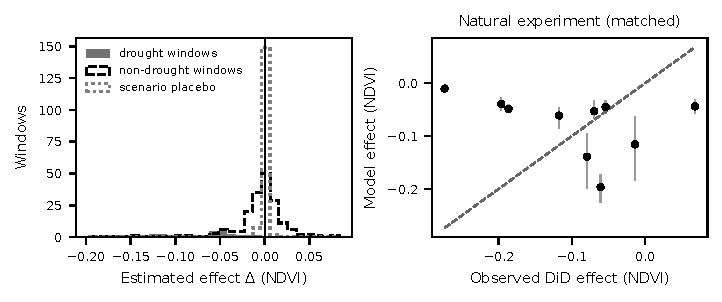
\includegraphics[width=\linewidth]{fig_validation.pdf}
\caption{Left: distribution of estimated effects (observed-weather minus normal-scenario forecast) for drought and
non-drought test windows, with the scenario placebo. Right: matched natural experiment (model effect vs.\ observed
difference-in-differences); only \V{diff_phys_G_P}{n_matched} treated windows could be matched.}
\label{fig:validation}\end{figure}
\paragraph{Observation-based checks.} On drought-labelled test windows the observed NDVI anomaly relative to
non-drought years at the same place and season is \D{obsanomdrought}. The physics-constrained model's anomaly is
\D{anom_ratio_diff_phys_G_P} times larger, unconstrained diffusion's \D{anom_ratio_diff_plain} times and the
deterministic network's \D{anom_ratio_det} times. Across windows, the model anomaly correlates weakly but
positively with the observed anomaly (\V{diff_phys_G_P}{anom_corr}, 95\,\% CI \V{diff_phys_G_P}{anom_corr_lo95} to
\V{diff_phys_G_P}{anom_corr_hi95}), so the model captures the direction of drought impacts but overstates their size.
In the cross-year proxy, the normal-scenario forecast change on drought windows
(MAE \V{diff_phys_G_P}{mae_normalD}) is further from the observed change in non-drought years than persistence
(\V{diff_phys_G_P}{mae_persistenceD}) and climatology (\V{diff_phys_G_P}{mae_climatologyD}). The natural
experiment is uninformative under our pre-registered rule: \V{diff_phys_G_P}{n_matched} pairs could be matched,
but with covariate imbalance above the 0.25 limit (maximum standardised mean difference
\V{diff_phys_G_P}{max_abs_smd}). With fewer than three informative observation-based checks, the drought-effect claim
is rated \emph{insufficient evidence}.
\paragraph{Sanity checks.} Placebos behave as expected (two different normal-analog assignments give a mean effect of
\V{diff_phys_G_P}{scenario_placebo_mean}), and common random numbers reduce the variance of $\Delta$ to a fraction
\V{diff_phys_G_P}{crn_var_ratio} of the independent-noise variance. These checks rely on model inputs only and cannot
establish credibility.
\paragraph{Calibration.} Ensembles remain overconfident after the validation-fitted spread correction: the central
90\,\% interval covers \R{diff_phys_G_P}{cov90} of observations (seeds 1 and 2: \R{diff_phys_G_P}{cov90s1},
\R{diff_phys_G_P}{cov90s2}) and the spread--skill ratio is \R{diff_phys_G_P}{spread_skill}. A spread--skill ratio
close to 1 with low coverage points to a property of small ensembles: the empirical 5--95\,\% interval of $M$
members cannot reach nominal coverage even for a perfectly calibrated ensemble (the full range $[\min,\max]$ covers on
average only $(M-1)/(M+1)$, i.e.\ 78\,\% for $M=8$). The pre-registered calibration verdict uses 8 members and is
therefore partly a consequence of ensemble size (Section~\ref{sec:confirm}).

\section{Confirmation on reserved test locations}\label{sec:confirm}
After the main evaluation, we evaluated the same models once on \CF{nloctest}{all} further fresh test locations that
had been left out at the main deadline and were seen by no model. The design, including a post-hoc calibration
(per-lead bias correction and spread factor fitted on validation data), was committed before any result. With 8
members and no correction, the replication reproduces the main findings: the physical-consistency claim is
supported in all three seeds, the physics model is closer to the observed sharpness than the deterministic network in
all three seeds, CRPS accuracy is again only partly supported, and 90\,\% coverage is again low
(\CF{diff_phys_G_P}{cov90s0}, \CF{diff_phys_G_P}{cov90s1}, \CF{diff_phys_G_P}{cov90s2}). The pre-registered calibrated
model with 32 members reaches 90\,\% coverage of \CF{diff_phys_G_P_Cal_m32}{cov90s0}, \CF{diff_phys_G_P_Cal_m32}{cov90s1}
and \CF{diff_phys_G_P_Cal_m32}{cov90s2}; it meets the calibration criterion in two of three seeds, so the verdict is
mixed. The bias correction, fitted on the validation year, did not transfer to the test years: it increased CRPS and
MAE. In an exploratory comparison (two of the three seeds added after seeing the first), the \emph{uncorrected}
model with 32 members reaches 90\,\% coverage of \CF{diff_phys_G_P_m32}{cov90s0}, \CF{diff_phys_G_P_m32}{cov90s1} and
\CF{diff_phys_G_P_m32}{cov90s2} with spread--skill ratios \CF{diff_phys_G_P_m32}{spread_skills2}--\CF{diff_phys_G_P_m32}{spread_skills1},
within the calibration criterion in all seeds. This indicates that the ensembles are reasonably calibrated and that
the main limitation was the ensemble size used for evaluation; because this comparison was not the pre-registered
primary analysis and uses only \CF{nloctest}{all} locations, we report it as exploratory.

\section{Limitations}
The drought effect is a model-based estimate, credible only if the model captures how weather drives vegetation and no
unobserved factor drives both. Weather is coarse (9--31\,km) relative to 20\,m imagery. This is a reduced-scale CPU
study: \D{nloc} locations, a small network, 5000 training steps, \D{nseeds} seeds and 8-member ensembles. Of the 80
planned fresh test locations, the \D{nloctest} whose downloads completed before a fixed deadline were used (decided
before any test result was seen). Bootstrap confidence intervals over \D{nloctest} location clusters may still be
too narrow, and only \D{neffdrought} drought-labelled test windows at \D{neffdroughtloc} locations were available for
the drought-effect analysis. The physics-loss weight scale was selected on validation from only three values.
Three earlier runs (69 and 80 locations, untuned and tuned) are reported in the repository; they agree in direction
but differ in the size of the drought-effect bias (archived results and \texttt{docs/LIMITATIONS.md}). The semi-synthetic oracle was
not run (real data only), and per-constraint retraining ablations were not run. See \texttt{docs/LIMITATIONS.md}.

\section{Conclusion}
Physics-constrained diffusion produced probabilistic NDVI forecasts that beat classical baselines and a deterministic
network in CRPS on fresh test locations, and its learned constraint losses consistently reduced physically
implausible behaviour across three training seeds without forcing violations to zero. The central hypothesis of credible
drought-attributable loss estimates is not established: model and observed drought anomalies agree in direction, but
the constrained models overstate drought losses (by a factor that differed between our runs), the natural experiment
is unbalanced. Apparent overconfidence of 8-member ensembles largely disappears with 32 members on reserved test
locations, although a pre-registered bias correction did not transfer across years. The validation framework, in particular the observation-based
anomaly and proxy checks, was essential to detect this; input-based placebos alone would have suggested success.
Larger training sets with more drought events, larger models trained longer, and constraints calibrated against
observed rather than idealised responses are the most important next steps.

\paragraph{Data and code availability.} Contains modified Copernicus Sentinel data (2017--2023) and modified
Copernicus Climate Change Service information. Weather data by Open-Meteo.com (CC BY 4.0). Produced using Copernicus
WorldDEM-30 \copyright\ DLR e.V. 2010--2014 and \copyright\ Airbus Defence and Space GmbH 2014--2018 provided under
COPERNICUS by the European Union and ESA; all rights reserved. \copyright\ ESA WorldCover project / Contains modified
Copernicus Sentinel data (2021) processed by ESA WorldCover consortium. Code: \url{https://github.com/Antony-Ahelgen/Counterfactual-Weather}.

\bibliographystyle{plain}
\bibliography{refs}
\end{document}
